%% =============================================================================
%% sm_e.tex — SM-E: Simulation and Computational Details (container file)
%% =============================================================================

This appendix provides computational and simulation details supplementing
\cref{sec:model,sec:simulation}.  \Cref{sme:model-hierarchy} presents the
five-model hierarchy with parameter counts.  \Cref{sme:mcmc} describes
the MCMC configuration and runtime benchmarks.  \Cref{smf:dgp} specifies
the data-generating process for the simulation study,
\cref{smf:diagnostics} presents supplementary simulation diagnostic
figures, \cref{smf:misspec} evaluates robustness under model
misspecification, \cref{smf:frequentist} provides a frequentist
contextualization, \cref{smf:decomposition} decomposes the coverage
gap into bias and width components, and \cref{smf:coverage95} reports
coverage at the 95\% nominal level.  Implementation details (non-centered parameterization,
numerical stability, score computation) are documented in the
\textsf{hurdlebb} package vignettes; full simulation results and
replication instructions are available in the replication package at
\url{https://github.com/joonho112/hurdlebb-replication}.

%% --- E.1: Model Hierarchy and Fitting Strategy (from old E.1) ---
%% =============================================================================
%% sm_e1_model_hierarchy.tex — SM-E, Subsection E.1: Model Hierarchy
%% Body content only (\subsection level); parent structure in sm_e.tex
%% =============================================================================

\subsection{Model hierarchy and architecture}
\label{sme:model-hierarchy}

\Cref{sme:tab-hierarchy} summarizes the five nested models fitted in
the application (\cref{sec:application}).  Each model extends its
predecessor by one structural feature: random intercepts (M1),
state-varying coefficients with block-diagonal covariance (M2),
cross-margin covariance (M3a), and policy moderators (M3b).  The
final model M3b-W adds survey weights to the pseudo-posterior.
Parameter counts include all fixed effects, random effects, and
hyperparameters (Cholesky factors, scales, and correlations).

The models are fitted sequentially using warm-start initialization:
the posterior mean of model~$k$ provides the initial values for
model~$k+1$.  Random-effect parameters absent in the simpler model
are initialized at zero (NCP variates) or identity (Cholesky factors).
This progressive strategy reduces total computation time by
approximately~$40\%$ compared with cold starts and ensures that each
model addresses a question raised by its predecessor:
M0 to M1 asks whether baseline enrolment rates vary by state;
M1 to M2, whether the poverty reversal varies by state;
M2 to M3a, whether cross-margin covariance improves fit;
and M3a to M3b, whether observable policies explain the state
heterogeneity.

\begin{table}[htbp]
  \centering
  \small
  \begin{tabular}{@{}l l r l r@{}}
    \toprule
    Model & Structure & Parameters
      & Covariance & $\widehat{\elpd}_{\mathrm{loo}}$ \\
    \midrule
    M0  & Pooled HBB
        & 11
        & ---
        & $-20{,}945$ \\
    M1  & Random intercepts
        & 116
        & $2 \times 2$
        & $-20{,}627$ \\
    M2  & Block-diagonal SVC
        & 551
        & $(5 \times 5) \oplus (5 \times 5)$
        & $-20{,}604$ \\
    M3a & Full SVC
        & 576
        & $10 \times 10$
        & $-20{,}602$ \\
    M3b & Policy moderators
        & 616
        & $10 \times 10$
        & $-20{,}608$ \\
    \bottomrule
  \end{tabular}
  \caption{Model hierarchy.  Parameters: total number of free
    parameters (fixed effects + random effects + hyperparameters).
    Covariance: dimension of the state-level covariance matrix for
    the random-effect deviations~$\bdelta_s$.  LOO: expected
    log-predictive density (\cref{sec:application}).  The
    progression from M0 to M3a yields significant incremental
    improvements in predictive accuracy; M3b adds policy
    moderators without further predictive gain.}
  \label{sme:tab-hierarchy}
\end{table}


%% --- E.2: MCMC Configuration (from old E.4) ---
%% =============================================================================
%% sm_e4_mcmc.tex — SM-E, Subsection E.4: MCMC Configuration
%% Body content only (\subsection level); parent structure in sm_e.tex
%% =============================================================================

\subsection{MCMC configuration}
\label{sme:mcmc}

All models are fitted using Stan
\citep{CarpenterEtAl2017} with the No-U-Turn Sampler
\citep[NUTS;][]{Hoffman2014} via the \textsf{CmdStanR} interface
\citep{CmdStanR2024}.  \Cref{sme:tab-mcmc} reports the sampler
configuration.

\begin{table}[htbp]
  \centering
  \begin{tabular}{@{}l ll@{}}
    \toprule
    Setting & Empirical (M0--M3b) & Simulation \\
    \midrule
    Chains                  & 4 (parallel) & 4 (parallel) \\
    Warmup iterations       & 1{,}000 per chain & 1{,}500 per chain \\
    Sampling iterations     & 1{,}000 per chain & 2{,}000 per chain \\
    Total post-warmup draws & 4{,}000 & 8{,}000 \\
    \texttt{adapt\_delta}    & 0.95 & 0.95 \\
    \texttt{max\_treedepth}  & 12 & 14 \\
    \bottomrule
  \end{tabular}
  \caption{MCMC configuration.  The empirical case study (M0--M3b)
    uses the default \textsf{hurdlebb} settings; the simulation study
    uses longer runs and higher \texttt{max\_treedepth} to ensure
    adequate exploration across 200 replications.  In both cases,
    \texttt{adapt\_delta} $= 0.95$ reduces the step size to avoid
    divergent transitions in the state-varying coefficient models.}
  \label{sme:tab-mcmc}
\end{table}

\paragraph{Convergence targets.}
As stated in~\cref{alg:estimation}, we require the following
diagnostic thresholds for all parameters~\citep{Vehtari2021}:
(i)~split-$\hat{R} < 1.01$;
(ii)~minimum bulk $\ESS > 400$;
(iii)~minimum tail $\ESS > 400$; and
(iv)~zero divergent transitions.
All five models satisfy these thresholds; detailed diagnostics
are available in the replication package.

\paragraph{Warm-start initialization.}
The five-model sequence M0 $\to$ M1 $\to$ M2 $\to$ M3a $\to$ M3b
is fitted progressively: the posterior mean from model~$k$ is used
to initialize model~$k+1$.  Specifically:
\begin{itemize}
  \item Fixed-effect coefficients ($\balpha$, $\bbeta$,
    $\log\kappa$) are initialized at the predecessor's posterior
    means.
  \item Scale parameters ($\boldsymbol{\tau}$) are initialized at the
    predecessor's posterior means when dimensions match, or at~$0.1$
    when new dimensions are introduced.
  \item Cholesky factors ($\mathbf{L}_\varepsilon$) are initialized at
    the identity matrix, which corresponds to zero correlation---a
    conservative starting point that lets the sampler discover
    correlations during warmup.
  \item NCP variates ($\bz_s$) are initialized at zero, placing all
    states at the global mean.
  \item Policy moderator coefficients ($\bGamma$, M3b only) are
    initialized at the predecessor's posterior means or at zero for
    newly introduced parameters.
\end{itemize}
This strategy avoids the slow exploration that can occur when complex
models are initialized far from the posterior mode.

\paragraph{Runtime benchmarks.}
On a 16-core workstation, approximate wall-clock times are:
M0~($\sim$5 minutes),
M1~($\sim$15 minutes),
M2~($\sim$30 minutes),
M3a~($\sim$50 minutes),
M3b~($\sim$60 minutes),
and M3b-W~($\sim$70 minutes, including score extraction in the
\texttt{generated quantities} block).  The total sequential fitting
time is approximately 4~hours with warm-start initialization, compared
to approximately 7~hours with cold starts.


%% --- E.3: Simulation Data-Generating Process (from old F.1) ---
%% =============================================================================
%% sm_f1_dgp.tex — SM-F, Subsection F.1: Data-Generating Process
%% Body content only (\subsection level); parent structure in sm_f.tex
%% =============================================================================

\subsection{Data-generating process and calibration}
\label{smf:dgp}

This section provides the complete data-generating process (DGP)
for the simulation study in~\cref{sec:simulation}.
The DGP is designed to match the NSECE 2019 data structure while
allowing parametric control over survey informativeness.

\paragraph{Population generation.}
A finite super-population of $M = 50{,}000$ providers is distributed
across $S = 51$ states, with state sizes proportional to the
observed NSECE state counts.  For each provider~$i$ in state~$s$:
\begin{enumerate}
  \item Draw the covariate vector
    $\bx_i = (1,\, x_{\mathrm{pov}},\, x_{\mathrm{urb}},\,
    x_{\mathrm{blk}},\, x_{\mathrm{his}})^\t$ by bootstrap
    resampling from the empirical NSECE marginals within state~$s$.
  \item Draw the trial size $n_i$ from the empirical distribution
    of total 0--5 enrollment in the NSECE data.
\end{enumerate}

\paragraph{True parameter values.}
The true parameters are calibrated to the M1 (random intercept)
unweighted NSECE fit (\cref{sme:model-hierarchy}).
\Cref{smf:tab-truth} reports all parameter values used in the
DGP.  These values were chosen to produce a realistic structural
zero rate (approximately 36\%) and overdispersion level
consistent with the empirical data.

\begin{table}[htbp]
  \centering
  \small
  \begin{tabular}{@{}l r l@{}}
    \toprule
    Parameter & Value & Description \\
    \midrule
    $\alpha_{\text{int}}$     & $+0.696$ & Extensive intercept \\
    $\alpha_{\text{pov}}$     & $-0.119$ & Extensive poverty \\
    $\alpha_{\text{urb}}$     & $+0.253$ & Extensive urban \\
    $\alpha_{\text{blk}}$     & $-0.070$ & Extensive Black \\
    $\alpha_{\text{his}}$     & $-0.139$ & Extensive Hispanic \\
    \addlinespace
    $\beta_{\text{int}}$      & $-0.032$ & Intensive intercept \\
    $\beta_{\text{pov}}$      & $+0.057$ & Intensive poverty \\
    $\beta_{\text{urb}}$      & $-0.018$ & Intensive urban \\
    $\beta_{\text{blk}}$      & $+0.080$ & Intensive Black \\
    $\beta_{\text{his}}$      & $+0.040$ & Intensive Hispanic \\
    \addlinespace
    $\log\kappa_0$            & $+1.655$ & Log concentration \\
    $\kappa_0$                & $5.232$ & Concentration \\
    \addlinespace
    $\tau_{\text{ext}}$       & $0.577$ & State SD (extensive) \\
    $\tau_{\text{int}}$       & $0.208$ & State SD (intensive) \\
    $\rho_{\text{cross}}$     & $0.285$ & Cross-margin correlation \\
    \bottomrule
  \end{tabular}
  \caption{True parameter values for the simulation DGP, calibrated to
    the M1 unweighted fit.  Fixed effects are on the logit scale;
    $\kappa_0 = \exp(\log\kappa_0)$.}
  \label{smf:tab-truth}
\end{table}

\paragraph{Outcome generation.}
For each replication~$r = 1,\ldots,R$:
\begin{enumerate}
  \item Draw state random effects
    $\bdelta_s = (\delta_{1s},\, \delta_{2s})^\t \sim
    \Norm_2(\mathbf{0}, \bSigma_\delta)$, where
    \[
      \bSigma_\delta = \diag(\boldsymbol{\tau})\,
      \mathbf{R}_\delta\,\diag(\boldsymbol{\tau}),
      \quad
      \boldsymbol{\tau} = (\tau_{\text{ext}},\,\tau_{\text{int}})^\t,
      \quad
      [\mathbf{R}_\delta]_{12} = \rho_{\text{cross}}.
    \]
  \item Compute linear predictors:
    $\eta_i^{\text{ext}} = \bx_i^\t\balpha_0 + \delta_{1,s[i]}$,
    $\eta_i^{\text{int}} = \bx_i^\t\bbeta_0 + \delta_{2,s[i]}$.
  \item Generate participation:
    $z_i \sim \Bern(q_i)$ with
    $q_i = \expit(\eta_i^{\text{ext}})$.
  \item For providers with $z_i = 1$, generate positive counts via
    \textbf{rejection sampling} from the unconditional beta-binomial
    \citep{Prentice1986}:
    \begin{quote}
      Draw $Y_i \sim \BetaBin(n_i,\, \mu_i,\, \kappa_0)$ where
      $\mu_i = \expit(\eta_i^{\text{int}})$;
      \emph{repeat until $Y_i > 0$}; set $y_i = Y_i$.
    \end{quote}
    This ensures $y_i > 0$ for all providers with $z_i = 1$,
    consistent with the zero-truncated beta-binomial component of
    the hurdle model.  The acceptance probability is $1 - p_0(n_i,
    \mu_i, \kappa_0)$, which exceeds~$0.80$ for the vast majority
    of observations in our calibration.
  \item For providers with $z_i = 0$, set $y_i = 0$.
\end{enumerate}

\begin{remark}[T3-3: Zero-truncated beta-binomial DGP]
  \label{smf:rem-ztbb}
  Drawing from the unconditional $\BetaBin$ and rejecting zeros
  produces exact draws from the zero-truncated beta-binomial
  $\ZTBB(n, \mu, \kappa)$.  The alternative---dividing the
  unconditional PMF by $(1-p_0)$---would require a custom
  sampling routine, whereas rejection sampling reuses the
  standard $\BetaBin$ sampler and is efficient whenever $p_0$ is
  not too close to~$1$.  The same approach is used in the
  Stan \texttt{generated quantities} block for posterior
  predictive replication.
\end{remark}

\paragraph{Sampling design.}
From each finite population, a stratified cluster sample of
approximately $N \approx 7{,}000$ providers is drawn using
size-biased inclusion probabilities
$\log\pi_i = c_0 + \rho_{\mathrm{inc}} \cdot y_i^*$
(\cref{eq:sim-inclusion}), where $y_i^*$ is the standardized
latent outcome and $c_0$ is calibrated to the target sample size
\citep[cf.][]{SavitskyToth2016}.
The three scenarios (S0, S3, S4) are defined in
\cref{tab:sim-scenarios}; see~\cref{sec:simulation} for the
full discussion.  Survey weights are computed as
$w_i = 1/\pi_i$ and normalized to sum to~$N$ for the
pseudo-posterior.


%% --- E.4: Supplementary Simulation Diagnostics (from old F.3) ---
%% =============================================================================
%% sm_f3_diagnostics.tex — SM-F, Subsection F.3: Supplementary Diagnostics
%% Body content only (\subsection level); parent structure in sm_f.tex
%% =============================================================================

\subsection{Supplementary diagnostic figures and design effect analysis}
\label{smf:diagnostics}

This section presents three supplementary figures that visualize
bias, interval width, and design effects across all simulation
scenarios, and a full table of design effect ratios (DER) for
all 11 fixed-effect parameters.

\paragraph{Relative bias distributions.}
\Cref{smf:fig-bias} shows the distribution of relative bias
across parameters and scenarios.  E-UW exhibits the largest
absolute bias (especially for $\tau_{\mathrm{ext}}$ and
$\tau_{\mathrm{int}}$ under S4), while E-WT/E-WS improve
point estimation for fixed effects by incorporating survey
weights.  For the poverty slopes $\alpha_{\mathrm{pov}}$ and
$\beta_{\mathrm{pov}}$, the relative bias under E-WS remains
below 15\% across all scenarios.

\begin{figure}[htbp]
  \centering
  
\includegraphics[width=0.95\textwidth]{SF7_simulation_bias.pdf}
  \caption{Relative bias (RB, \%) by parameter, estimator, and
    scenario.  Each panel corresponds to one of the five target
    parameters.  Dot positions indicate relative bias; color
    distinguishes scenarios (S0, S3, S4).  The vertical gray
    line marks zero bias.}
  \label{smf:fig-bias}
\end{figure}

\paragraph{Width ratio distributions.}
\Cref{smf:fig-wr} displays the distribution of width ratios
(WR = median CI width under E-WS / median CI width under E-WT)
across replications.  The progressive inflation from S0 through
S4 is clearly visible for all fixed-effect parameters.
The width ratio for $\log\kappa$ is similar to or slightly larger
than those for the poverty slopes, reflecting the nonlinear
dispersion score (Appendix~B).  Hyperparameter
width ratios are identically~$1.000$ (not shown) because no
sandwich correction is applied.

\begin{figure}[htbp]
  \centering
  
\includegraphics[width=0.95\textwidth]{SF8_width_ratio_distribution.pdf}
  \caption{Distribution of width ratios across $R = 200$
    replications, by parameter and scenario.  Boxplots are overlaid
    with violin plots to show the full distributional shape.  The
    horizontal dashed line at WR = 1.0 marks the no-correction
    reference.}
  \label{smf:fig-wr}
\end{figure}

\paragraph{Design effect ratios.}
\Cref{smf:fig-der} summarizes the simulation DER across all 11
fixed-effect parameters (5 extensive, 5 intensive, and
$\log\kappa$) and three scenarios.  The DER monotonically
increases with the informativeness parameter
$\rho_{\mathrm{inc}}$, consistent with the theoretical prediction
in~\cref{smc:prop-der-classification}.  Urban density parameters
exhibit the largest DER in all scenarios (mean 3.25 in S0 up to
6.43 in S4), mirroring the empirical DER of~4.18 for
$\alpha_{\mathrm{urb}}$ in the NSECE case study
(\cref{smd:tab-der}).

\begin{figure}[htbp]
  \centering
  
\includegraphics[width=0.95\textwidth]{SF9_DER_summary.pdf}
  \caption{Design effect ratios (DER) by parameter and scenario.
    Each dot represents the mean DER across 200 replications;
    color distinguishes scenarios.  Parameters are grouped by
    margin (extensive vs.\ intensive) with $\log\kappa$ as a
    separate category.}
  \label{smf:fig-der}
\end{figure}

\paragraph{Complete DER table.}
The table below reports the full distribution of DER across
replications for all 11 fixed-effect parameters and three
scenarios.  The mean, median, standard deviation, and range
(min--max) characterize the replication-to-replication
variability.  Two patterns are noteworthy: (i)~the DER standard
deviation increases with the scenario severity, indicating
greater sampling variability under heavier design effects; and
(ii)~the urban parameter consistently shows the widest DER
range, reflecting the spatial concentration of urban providers
that amplifies the design effect.

{\small
% latex table generated in R 4.5.1 by xtable 1.8-4 package
% Mon Feb 23 11:13:23 2026
\begin{table}[htbp]
\centering
\begin{tabular}{llrlllllll}
  \toprule
Scenario & Parameter & R & Mean & Median & SD & Min & Q25 & Q75 & Max \\ 
  \midrule
S0: Non-informative & Intercept (ext) & 200 & 1.99 & 1.95 & 0.28 & 1.29 & 1.80 & 2.16 & 2.92 \\ 
  S0: Non-informative & Poverty (ext) & 200 & 1.90 & 1.89 & 0.32 & 1.23 & 1.67 & 2.09 & 3.07 \\ 
  S0: Non-informative & Urban (ext) & 200 & 3.25 & 3.18 & 0.69 & 1.59 & 2.74 & 3.68 & 5.28 \\ 
  S0: Non-informative & Black (ext) & 200 & 2.08 & 2.05 & 0.36 & 1.14 & 1.83 & 2.29 & 3.46 \\ 
  S0: Non-informative & Hispanic (ext) & 200 & 1.69 & 1.67 & 0.24 & 1.05 & 1.54 & 1.80 & 2.68 \\ 
  S0: Non-informative & Intercept (int) & 200 & 2.00 & 1.97 & 0.30 & 1.38 & 1.79 & 2.17 & 2.92 \\ 
  S0: Non-informative & Poverty (int) & 200 & 1.81 & 1.80 & 0.31 & 1.06 & 1.62 & 1.96 & 3.11 \\ 
  S0: Non-informative & Urban (int) & 200 & 2.93 & 2.86 & 0.70 & 1.41 & 2.44 & 3.33 & 5.35 \\ 
  S0: Non-informative & Black (int) & 200 & 2.07 & 2.02 & 0.39 & 1.32 & 1.77 & 2.28 & 3.55 \\ 
  S0: Non-informative & Hispanic (int) & 200 & 1.61 & 1.59 & 0.23 & 1.11 & 1.45 & 1.76 & 2.34 \\ 
  S0: Non-informative & log kappa & 200 & 1.73 & 1.71 & 0.27 & 1.12 & 1.55 & 1.92 & 2.36 \\ 
  S3: NSECE-calibrated & Intercept (ext) & 200 & 4.02 & 3.88 & 0.97 & 1.97 & 3.29 & 4.71 & 7.47 \\ 
  S3: NSECE-calibrated & Poverty (ext) & 200 & 3.79 & 3.72 & 0.97 & 1.90 & 3.03 & 4.45 & 7.53 \\ 
  S3: NSECE-calibrated & Urban (ext) & 200 & 5.55 & 5.43 & 1.72 & 1.62 & 4.31 & 6.56 & 11.21 \\ 
  S3: NSECE-calibrated & Black (ext) & 200 & 4.01 & 3.81 & 1.09 & 2.07 & 3.13 & 4.64 & 7.23 \\ 
  S3: NSECE-calibrated & Hispanic (ext) & 200 & 3.03 & 2.94 & 0.73 & 1.58 & 2.50 & 3.50 & 5.26 \\ 
  S3: NSECE-calibrated & Intercept (int) & 200 & 3.80 & 3.70 & 0.88 & 1.68 & 3.13 & 4.46 & 6.40 \\ 
  S3: NSECE-calibrated & Poverty (int) & 200 & 3.44 & 3.42 & 0.89 & 1.53 & 2.79 & 3.89 & 7.32 \\ 
  S3: NSECE-calibrated & Urban (int) & 200 & 5.34 & 5.26 & 1.41 & 2.34 & 4.41 & 6.13 & 11.40 \\ 
  S3: NSECE-calibrated & Black (int) & 200 & 3.89 & 3.67 & 1.10 & 1.96 & 3.19 & 4.52 & 7.45 \\ 
  S3: NSECE-calibrated & Hispanic (int) & 200 & 2.72 & 2.65 & 0.63 & 1.67 & 2.20 & 3.09 & 5.16 \\ 
  S3: NSECE-calibrated & log kappa & 200 & 3.12 & 3.07 & 0.69 & 1.38 & 2.74 & 3.55 & 5.44 \\ 
  S4: Stress test & Intercept (ext) & 200 & 5.50 & 5.23 & 1.52 & 2.79 & 4.45 & 6.10 & 13.23 \\ 
  S4: Stress test & Poverty (ext) & 200 & 5.51 & 5.31 & 1.51 & 2.72 & 4.37 & 6.48 & 11.59 \\ 
  S4: Stress test & Urban (ext) & 200 & 6.43 & 6.22 & 1.91 & 2.97 & 5.07 & 7.66 & 17.11 \\ 
  S4: Stress test & Black (ext) & 200 & 5.75 & 5.41 & 1.75 & 2.30 & 4.45 & 6.79 & 11.38 \\ 
  S4: Stress test & Hispanic (ext) & 200 & 4.46 & 4.36 & 1.14 & 1.91 & 3.70 & 5.02 & 10.86 \\ 
  S4: Stress test & Intercept (int) & 200 & 4.86 & 4.71 & 1.26 & 2.38 & 3.93 & 5.52 & 9.53 \\ 
  S4: Stress test & Poverty (int) & 200 & 4.66 & 4.44 & 1.39 & 2.31 & 3.60 & 5.45 & 9.04 \\ 
  S4: Stress test & Urban (int) & 200 & 6.11 & 5.96 & 1.74 & 2.24 & 5.02 & 7.15 & 13.79 \\ 
  S4: Stress test & Black (int) & 200 & 5.19 & 5.01 & 1.48 & 2.13 & 4.16 & 5.98 & 10.13 \\ 
  S4: Stress test & Hispanic (int) & 200 & 3.84 & 3.74 & 0.95 & 1.78 & 3.07 & 4.57 & 6.44 \\ 
  S4: Stress test & log kappa & 200 & 4.21 & 4.10 & 1.06 & 2.11 & 3.50 & 4.85 & 7.69 \\ 
   \bottomrule
\end{tabular}
\caption{Design Effect Ratios (DER) Across Simulation Replications. DER = diag($V_{\text{sand}}$) / diag($H_{\text{obs}}^{-1}$). All 11 fixed-effect parameters shown.} 
\end{table}

}

\paragraph{Cross-margin correlation recovery.}
\cref{tab:rho-cross-sim} reports recovery of the cross-margin
correlation $\rho_{\mathrm{cross}} = \operatorname{cor}(\delta_j^{\mathrm{ext}},
\delta_j^{\mathrm{int}})$ using a plug-in estimator based on posterior
mean random effects across $S = 51$ states.
The unweighted estimator E-UW systematically overestimates
$\rho_{\mathrm{cross}}$, with relative bias growing from $+84\%$ in
S0 to $+127\%$ in S4.
The weighted estimator E-WT shows moderate downward bias ($-26\%$ to
$-45\%$), and E-WS is identical to E-WT because the Cholesky sandwich
correction (\cref{thm:cholesky}) adjusts only fixed-effect covariances.
Per-replication credible intervals are unavailable because full
posterior draws of the correlation matrix $\Omega$ were not retained
in the simulation archive; only frequentist summaries across
replications are reported.

{\small
\begin{table}[t]
\centering
\caption{Recovery of the cross-margin correlation $\rho_{\mathrm{cross}} = \operatorname{cor}(\delta_j^{\mathrm{ext}}, \delta_j^{\mathrm{int}})$
  across $R = 200$ simulation replications. The plug-in estimator 
  $\hat{\rho} = \operatorname{cor}(\bar{\delta}_j^{\mathrm{ext}}, \bar{\delta}_j^{\mathrm{int}})$
  uses posterior mean random effects ($S = 51$ states). True value: $\rho_{\mathrm{cross}} = 0.2853$.
  E\textsubscript{WS} is identical to E\textsubscript{WT} because the sandwich correction applies only to fixed effects.}
\label{tab:rho-cross-sim}
\smallskip
\small
\begin{tabular}{@{}ll rrrrr@{}}
\toprule
Scenario & Estimator & $\overline{\hat{\rho}}$ & Bias & Rel.~Bias (\%) & RMSE & Emp.~SE \\
\midrule
S0 (Baseline)      & E\textsubscript{UW}                 & 0.5238 & $+0.2386$ & $+83.6$ & 0.2990 & 0.1807 \\
                   & E\textsubscript{WT}                 & 0.2104 & $-0.0749$ & $-26.3$ & 0.2294 & 0.2173 \\
                   & E\textsubscript{WS}$^{\dagger}$     & 0.2104 & $-0.0749$ & $-26.3$ & 0.2294 & 0.2173 \\
\midrule
S3 (NSECE)         & E\textsubscript{UW}                 & 0.5814 & $+0.2961$ & $+103.8$ & 0.3643 & 0.2128 \\
                   & E\textsubscript{WT}                 & 0.1658 & $-0.1195$ & $-41.9$ & 0.2256 & 0.1918 \\
                   & E\textsubscript{WS}$^{\dagger}$     & 0.1658 & $-0.1195$ & $-41.9$ & 0.2256 & 0.1918 \\
\midrule
S4 (Heavy-tail)    & E\textsubscript{UW}                 & 0.6468 & $+0.3615$ & $+126.7$ & 0.4075 & 0.1886 \\
                   & E\textsubscript{WT}                 & 0.1579 & $-0.1274$ & $-44.7$ & 0.2372 & 0.2005 \\
                   & E\textsubscript{WS}$^{\dagger}$     & 0.1579 & $-0.1274$ & $-44.7$ & 0.2372 & 0.2005 \\
\bottomrule
\end{tabular}

\medskip
{\footnotesize $^{\dagger}$E\textsubscript{WS} shares the same Stan fit as E\textsubscript{WT}; the Cholesky sandwich correction adjusts only fixed-effect covariances, not hyperparameter posteriors.}
\end{table}

}


%% --- E.5: Model Misspecification Robustness ---
%% =============================================================================
%% sm_f5_misspec.tex — SM-E, Subsection E.5: Misspecification Robustness
%% Body content only (\subsection level); parent structure in sm_e.tex
%% =============================================================================

\subsection{Model misspecification robustness}
\label{smf:misspec}

The simulation study in \cref{sec:simulation} evaluates the
correctly specified case: data are generated from the random-intercept
model~M1 and fitted by M1.  A natural concern is how the three
estimators (E-UW, E-WT, E-WS) behave when the fitted model omits a
relevant source of heterogeneity.  We therefore augment the simulation
with a misspecification scenario designed to probe whether the sandwich
correction remains beneficial when the model is wrong.

\paragraph{M2 data-generating process.}
Define the \emph{state-varying coefficient} DGP~(M2) by
adding random poverty slopes to the M1 linear predictors:
\begin{align}
  \eta^{\mathrm{ext}}_i &= \bx_i^\t \balpha + \delta^{\mathrm{ext}}_{s[i]}
    + \gamma^{\mathrm{ext}}_{s[i]} \, x_{\mathrm{pov},i}, \label{eq:m2-ext}\\
  \eta^{\mathrm{int}}_i &= \bx_i^\t \bbeta  + \delta^{\mathrm{int}}_{s[i]}
    + \gamma^{\mathrm{int}}_{s[i]} \, x_{\mathrm{pov},i}, \label{eq:m2-int}
\end{align}
where $\gamma^{\mathrm{ext}}_s \sim \Norm(0, 0.15^2)$ and
$\gamma^{\mathrm{int}}_s \sim \Norm(0, 0.10^2)$ independently across
$s = 1,\ldots,51$ states.  All other parameters
($\balpha, \bbeta, \kappa, \boldsymbol{\tau}, \rho$) and the population structure
($M = 50{,}000$ providers) are identical to the M1 DGP
(\cref{smf:dgp}).  The standard deviations $0.15$ (extensive) and
$0.10$ (intensive) produce state-varying poverty effects that are
moderate relative to the fixed poverty coefficients
($\alpha_{\mathrm{pov}} = -0.119$, $\beta_{\mathrm{pov}} = +0.057$).

\paragraph{Design.}
We draw $R = 200$ independent replications under the S3
(NSECE-calibrated) informativeness scenario with
$\operatorname{DEFF} \approx 3.79$, and fit the M1 random-intercept
model using all three estimators.  The M1 fit ignores the
state-varying poverty slopes $\gamma_s$, inducing a form of
omitted-variable misspecification that propagates through the
poverty coefficient estimates.

\paragraph{Results.}
\Cref{smf:tab-misspec} compares coverage, relative bias, RMSE, and
width ratio for the correctly specified S3 scenario (M1 truth, M1 fit)
and the misspecified B5 scenario (M2 truth, M1 fit).
%% NOTE: Table and figure placeholders below will be populated by
%% 85_B5_misspec_analysis.R once simulation results are collected.

\begin{table}[htbp]
\centering
\caption{Misspecification robustness: correctly specified S3 vs.\
  misspecified B5 (M2 truth, M1 fit) under NSECE-calibrated
  sampling ($\operatorname{DEFF} \approx 3.79$).
  $R = 200$ replications; nominal coverage $= 90\%$;
  $\dagger$ indicates significant departure ($> 2 \times$ MCSE).
  MCSE $= \sqrt{\hat{p}(1-\hat{p})/200}$; range 0.0--3.5 pp.}
\label{smf:tab-misspec}
% Generated by 85_B5_misspec_analysis.R — B5 misspecification robustness
% S3 = correctly specified (M1 truth, M1 fit); B5 = misspecified (M2 truth, M1 fit)
\small
\begin{adjustbox}{max width=\textwidth}
\begin{tabular}{@{}l l rr rrr rrr rr@{}}
\toprule
 & & \multicolumn{2}{c}{Coverage (\%)} &
     \multicolumn{3}{c}{Relative bias (\%)} &
     \multicolumn{3}{c}{RMSE} &
     \multicolumn{2}{c}{WR} \\
\cmidrule(lr){3-4}\cmidrule(lr){5-7}\cmidrule(lr){8-10}\cmidrule(lr){11-12}
Parameter & Est. & S3 & B5 & S3 & B5 & $\Delta$ &
  S3 & B5 & $\Delta$ & S3 & B5 \\
\midrule
\multicolumn{12}{@{}l}{\textit{Fixed effects}} \\[2pt]
$\alpha_{\text{pov}}$ & E-UW & 89.5 & 0.5$^{\dagger}$ &
  $+$16.5 & $-$117.8 & $-$134.3 & 0.037 & 0.143 & $+$0.106 & --- & --- \\
 & E-WT & 58.5$^{\dagger}$ & 52.0$^{\dagger}$ &
  $+$12.9 & $-$37.6 & $-$50.5 & 0.072 & 0.079 & $+$0.007 & --- & --- \\
 & E-WS & 82.0$^{\dagger}$ & 79.0$^{\dagger}$ &
  $+$12.9 & $-$37.6 & $-$50.5 & 0.072 & 0.079 & $+$0.007 & 1.71 & 1.67 \\[3pt]
$\beta_{\text{pov}}$ & E-UW & 89.0 & 30.0$^{\dagger}$ &
  $-$16.7 & $+$63.1 & $+$79.8 & 0.017 & 0.039 & $+$0.022 & --- & --- \\
 & E-WT & 62.5$^{\dagger}$ & 42.0$^{\dagger}$ &
  $-$3.2 & $+$52.7 & $+$55.9 & 0.032 & 0.043 & $+$0.011 & --- & --- \\
 & E-WS & 82.5$^{\dagger}$ & 67.5$^{\dagger}$ &
  $-$3.2 & $+$52.7 & $+$55.9 & 0.032 & 0.043 & $+$0.011 & 1.64 & 1.60 \\[3pt]
$\log\kappa$ & E-UW & 92.0 & 82.5$^{\dagger}$ &
  $-$0.5 & $-$1.3 & $-$0.8 & 0.020 & 0.027 & $+$0.007 & --- & --- \\
 & E-WT & 34.0$^{\dagger}$ & 36.5$^{\dagger}$ &
  $+$3.3 & $+$2.9 & $-$0.4 & 0.068 & 0.064 & $-$0.004 & --- & --- \\
 & E-WS & 60.5$^{\dagger}$ & 64.0$^{\dagger}$ &
  $+$3.3 & $+$2.9 & $-$0.4 & 0.068 & 0.064 & $-$0.004 & 1.75 & 1.74 \\[4pt]
\multicolumn{12}{@{}l}{\textit{Variance components}} \\[2pt]
$\tau_{\text{ext}}$ & E-UW & 98.0$^{\dagger}$ & 96.0$^{\dagger}$ &
  $+$8.0 & $-$2.5 & $-$10.5 & 0.091 & 0.117 & $+$0.026 & --- & --- \\
 & E-WT & 0.5$^{\dagger}$ & 0.0$^{\dagger}$ &
  $+$105.6 & $+$102.4 & $-$3.2 & 0.639 & 0.625 & $-$0.014 & --- & --- \\
 & E-WS & 0.5$^{\dagger}$ & 0.0$^{\dagger}$ &
  $+$105.6 & $+$102.4 & $-$3.2 & 0.639 & 0.625 & $-$0.014 & 1.00 & 1.00 \\[3pt]
$\tau_{\text{int}}$ & E-UW & 97.5$^{\dagger}$ & 57.0$^{\dagger}$ &
  $-$8.6 & $-$34.8 & $-$26.2 & 0.040 & 0.079 & $+$0.039 & --- & --- \\
 & E-WT & 0.0$^{\dagger}$ & 1.0$^{\dagger}$ &
  $+$97.6 & $+$97.0 & $-$0.6 & 0.211 & 0.213 & $+$0.002 & --- & --- \\
 & E-WS & 0.0$^{\dagger}$ & 1.0$^{\dagger}$ &
  $+$97.6 & $+$97.0 & $-$0.6 & 0.211 & 0.213 & $+$0.002 & 1.00 & 1.00 \\
\bottomrule
\end{tabular}
\end{adjustbox}

\end{table}

\Cref{smf:fig-misspec-coverage} displays the corresponding coverage
rates graphically.

\begin{figure}[htbp]
\centering
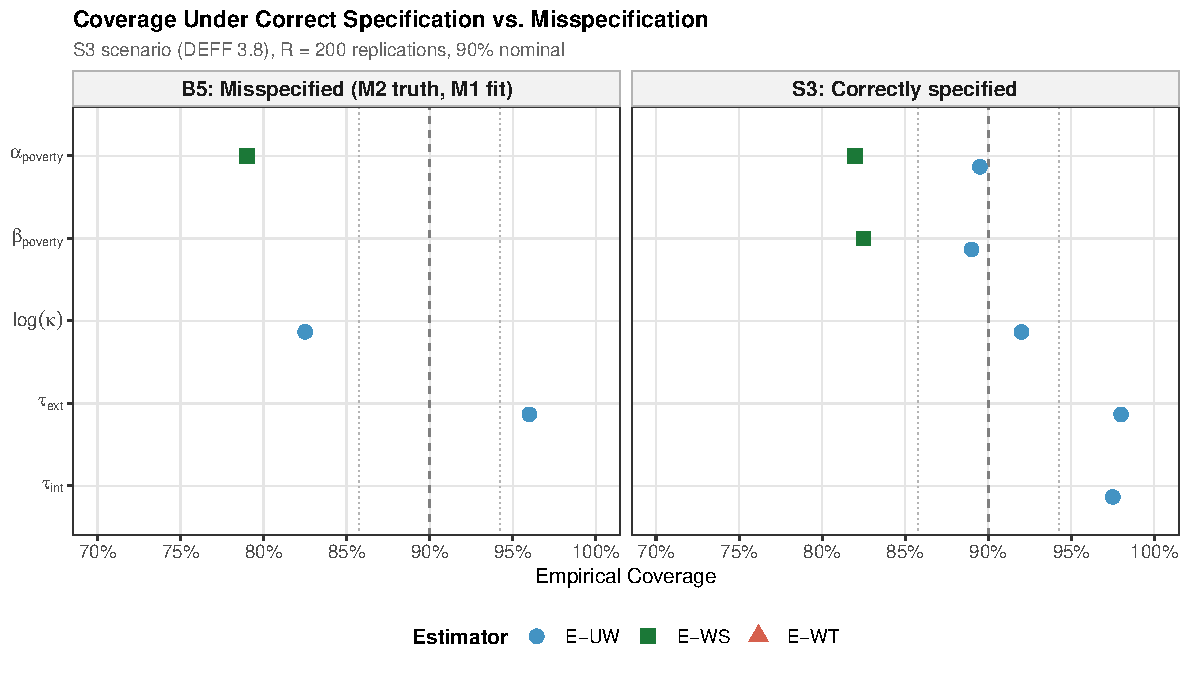
\includegraphics[width=\textwidth]{Figures/SF_B5_misspec_coverage}
\caption{Coverage under correct specification (S3) vs.\
  misspecification (B5).  Vertical dashed line: 90\% nominal;
  dotted lines: $\pm 2\,\mathrm{MCSE}$ band.}
\label{smf:fig-misspec-coverage}
\end{figure}

Three findings emerge from the comparison.

\paragraph{Finding B5-1: The unweighted estimator is acutely sensitive
to misspecification in the poverty coefficients.}
Under correct specification (S3), E-UW achieves near-nominal coverage
for both poverty slopes (89.5\% and 89.0\%).  Under the M2 DGP, E-UW
coverage collapses to 0.5\% for $\alpha_{\mathrm{pov}}$ and 30.0\%
for $\beta_{\mathrm{pov}}$---drops of 89 and 59 percentage points,
respectively.  The mechanism is omitted-variable bias: because M1
lacks the state-varying poverty slopes $\gamma_s$, the fixed
coefficients $\alpha_{\mathrm{pov}}$ and $\beta_{\mathrm{pov}}$ absorb
the omitted heterogeneity, producing relative bias of $-117.8\%$ and
$+63.1\%$.  This confirms that the model-based intervals of E-UW are
valid only under correct specification---a strong argument for the
design-based protection that survey weighting provides.

\paragraph{Finding B5-2: The sandwich correction preserves coverage
stability under misspecification.}
For $\alpha_{\mathrm{pov}}$, E-WS coverage declines only from 82.0\%
(S3) to 79.0\% (B5)---a 3-percentage-point drop---while E-WT drops
from 58.5\% to 52.0\%.  For $\beta_{\mathrm{pov}}$, E-WS declines
from 82.5\% to 67.5\% ($-15$ pp) compared with E-WT's drop from
62.5\% to 42.0\% ($-20.5$ pp).  In both cases, E-WS maintains a
substantial advantage over E-WT (27 and 25.5 percentage points under
B5), demonstrating that the sandwich variance correction absorbs a
meaningful share of the misspecification-induced variance increase.
The width ratios remain stable across scenarios
($\mathrm{WR} = 1.67\text{--}1.74$ under B5 vs.\ $1.64\text{--}1.75$
under S3), indicating that the design effect magnitude is similar
regardless of whether the model is correctly specified.

\paragraph{Finding B5-3: Variance components exhibit differential
sensitivity.}
The overdispersion $\log\kappa$ is relatively robust under E-UW
(coverage 92.0\% $\to$ 82.5\%; relative bias $-0.5\%$ $\to$ $-1.3\%$),
as expected since the omitted random slopes do not directly affect the
dispersion structure.  Among the variance components,
$\tau_{\mathrm{ext}}$ remains well-covered under E-UW (98.0\% $\to$
96.0\%), but $\tau_{\mathrm{int}}$ drops sharply (97.5\% $\to$
57.0\%).  The asymmetry arises because the omitted intensive-margin
slopes ($\sigma_{\gamma}^{\mathrm{int}} = 0.10$ relative to
$\tau_{\mathrm{int}} = 0.208$) contribute proportionally more
unmodeled between-state variance than the extensive-margin slopes
($\sigma_{\gamma}^{\mathrm{ext}} = 0.15$ relative to
$\tau_{\mathrm{ext}} = 0.577$).  As in the correctly specified case,
E-WT and E-WS produce near-zero coverage for both $\tau$ parameters
($\mathrm{WR} = 1.00$), reaffirming that the sandwich correction is
structurally inapplicable to variance components.

Taken together, these results strengthen the case for the two-track
reporting strategy recommended in~\cref{sec:simulation}: for
population-average fixed effects, the sandwich-corrected estimator
E-WS provides meaningful robustness against model misspecification;
for hierarchical variance components, the unweighted estimator E-UW
remains the only viable option, with the caveat that its validity
depends on correct specification of the random-effects structure.


%% --- E.6: Frequentist Contextualization ---
%% =============================================================================
%% sm_f6_frequentist.tex — SM-E, Subsection E.6: Frequentist Contextualization
%% Body content only (\subsection level); parent structure in sm_e.tex
%% =============================================================================

\subsection{Frequentist contextualization}
\label{smf:frequentist}

A natural question is whether a simpler design-based analysis could
replace the full Bayesian hierarchical model.  We compare the HBB
pseudo-posterior estimates with conventional survey-weighted frequentist
estimates obtained from \texttt{survey::svyglm}
\citep{Lumley2004,Lumley2020} to (i)~validate the design-consistency
of the pseudo-posterior fixed effects and (ii)~clarify which model
features cannot be accommodated by the frequentist approach.

\paragraph{Frequentist specification.}
We fit separate margin models using the same five-covariate
specification as the HBB model.  For the extensive margin, we fit a
survey-weighted logistic regression using
\texttt{svyglm(\ldots, family = quasibinomial())} with $N = 6{,}785$
observations.  For the intensive margin, we fit a survey-weighted
linear regression of the IT enrollment share $y_i / n_i$ on the same
covariates, restricted to the $N^{+} = 4{,}392$ participants.  Both
models use the NSECE complex survey design (stratification, clustering,
and sampling weights) and produce linearization-based cluster-robust
standard errors.  No random effects, beta-binomial structure, or
cross-margin dependence can be incorporated.

\paragraph{Results.}
\Cref{smf:tab-frequentist} compares the survey-weighted svyglm
estimates with the M3b-W sandwich-corrected pseudo-posterior summaries.

\begin{table}[htbp]
\centering
\caption{Frequentist contextualization: survey-weighted svyglm vs.\
  Bayesian HBB (M3b-W, sandwich-corrected) point estimates and standard
  errors.  The extensive margin uses logistic link in both approaches;
  the intensive margin uses an identity link (svyglm) vs.\ logit link
  (HBB), so the scales differ.  SE Ratio $=$ HBB sandwich SE / svyglm SE.}
\label{smf:tab-frequentist}
% Generated by 86_B6_frequentist_comparison.R
\small
\begin{adjustbox}{max width=\textwidth}
\begin{tabular}{@{}l l rr rr r r@{}}
\toprule
 & & \multicolumn{2}{c}{svyglm (design-based)} &
   \multicolumn{2}{c}{HBB (sandwich-corrected)} & & \\
\cmidrule(lr){3-4}\cmidrule(lr){5-6}
Margin & Parameter & Est. & SE & Est. & SE & $\Delta$Est. & SE Ratio \\
\midrule
Extensive & Intercept & 0.662 & 0.063 & 0.764 & 0.044 & +0.103 & 0.70 \\
 & Poverty & -0.199 & 0.071 & -0.324 & 0.052 & -0.125 & 0.74 \\
 & Urban & 0.234 & 0.039 & 0.442 & 0.034 & +0.208 & 0.89 \\
 & Black & 0.086 & 0.075 & 0.478 & 0.044 & +0.392 & 0.59 \\
 & Hispanic & 0.059 & 0.074 & 0.006 & 0.051 & -0.054 & 0.70 \\
[3pt]
Intensive & Intercept & 0.483 & 0.005 & -0.242 & 0.015 & -0.725 & 3.02 \\
 & Poverty & 0.015 & 0.007 & 0.090 & 0.019 & +0.075 & 2.77 \\
 & Urban & -0.009 & 0.004 & -0.047 & 0.021 & -0.038 & 4.63 \\
 & Black & 0.034 & 0.008 & -0.017 & 0.018 & -0.050 & 2.30 \\
 & Hispanic & 0.010 & 0.006 & -0.097 & 0.017 & -0.107 & 2.92 \\
\bottomrule
\end{tabular}
\end{adjustbox}

\end{table}

For the extensive margin, both approaches use the logit link, enabling
a meaningful comparison on a common scale.  The coefficient signs and
relative magnitudes agree across all five predictors.  Point estimates
from HBB are systematically larger in absolute value than the svyglm
estimates, which is expected: the HBB model conditions on state-level
random effects, and conditional effects in mixed models are known to
exceed their marginal counterparts
\citep{ZegerLiangAlbert1988}.  The SE ratio
(HBB sandwich / svyglm) ranges from $0.59$ to $0.89$, reflecting the
variance reduction achieved by modeling between-state heterogeneity
through random effects rather than absorbing it into the residual.

For the intensive margin, the comparison is less direct because the two
approaches operate on different scales: svyglm regresses the
enrollment share $y_i / n_i$ under an identity link, while HBB models
the beta-binomial mean parameter $\mu_i$ under a logit link.  The
differing intercepts (svyglm: $+0.483$; HBB: $-0.242$) reflect this
scale difference rather than substantive disagreement, since
$\operatorname{logit}^{-1}(-0.242) \approx 0.44$, which is in the
range of the observed mean share.  The larger SE ratios for the
intensive margin ($2.30$--$4.63$) also arise from the logit-scale
parameterization, which inflates variances relative to the probability
scale.

\paragraph{Structural limitations.}
The comparison highlights several features of the HBB framework
that \texttt{svyglm} cannot accommodate:
\begin{enumerate}[nosep]
  \item \emph{Beta-binomial distribution:} svyglm models the continuous
    share $y/n$ via Gaussian errors, ignoring the bounded-count nature of
    the outcome and the extra-binomial overdispersion ($\kappa = 6.81$).
  \item \emph{Hurdle structure:} the two margins must be fitted
    separately, precluding joint inference on the zero-generating process.
  \item \emph{State-level random effects:} svyglm is a fixed-effect
    estimator; accommodating $S = 51$ state intercepts (and slopes in M3b)
    would require either fixed-effect dummies---inflating SE and
    sacrificing shrinkage---or a two-step approach that does not
    propagate uncertainty.
  \item \emph{Cross-margin correlation:} the bivariate random-effect
    structure $\boldsymbol{\delta}_s \sim \Norm_{2q}(\mathbf{0},
    \boldsymbol{\Sigma}_\delta)$ cannot be replicated in separate
    margin-specific regressions.
  \item \emph{Policy moderation:} the state-varying policy coefficients
    $\boldsymbol{\Gamma}$ interact hierarchical and design-based
    components in a way that has no natural frequentist counterpart.
\end{enumerate}

Taken together, the svyglm comparison serves as a fixed-effect-level
sanity check: the Bayesian pseudo-posterior fixed effects are
design-consistent with the frequentist target, while the full HBB
framework adds hierarchical structure, distributional flexibility,
and joint inference that the frequentist alternative cannot provide.


%% --- E.7: Coverage Gap Decomposition ---
%% =============================================================================
%% sm_f7_decomposition.tex — SM-E, Subsection E.7: Coverage Gap Decomposition
%% Body content only (\subsection level); parent structure in sm_e.tex
%% =============================================================================

\subsection{Coverage gap decomposition}
\label{smf:decomposition}

\Cref{smf:tab-decomposition} decomposes the coverage gap for each
parameter--estimator combination under the S3 (NSECE-calibrated) scenario.
Two diagnostic quantities distinguish width-driven from bias-driven
shortfalls:
\begin{itemize}[nosep]
  \item \emph{SE calibration ratio} $= \widehat{\mathrm{SD}} /
    \overline{\mathrm{SE}}$, where $\widehat{\mathrm{SD}}$ is the
    empirical standard deviation of point estimates across $R = 200$
    replications and $\overline{\mathrm{SE}}$ is the mean reported
    standard error.  A ratio exceeding 1 indicates that the reported SE
    underestimates the actual sampling variability (width-driven gap).
  \item \emph{Standardized mean bias} $= |\bar{b}| /
    \widehat{\mathrm{SD}}$, where $\bar{b}$ is the mean bias across
    replications.  Values exceeding $\sim 0.5$ indicate non-negligible
    centering error (bias-driven gap).
\end{itemize}

\begin{table}[htbp]
\centering
\caption{Coverage gap decomposition under the S3 (NSECE-calibrated)
  scenario.  ``Below'' and ``Above'' report the percentage of replications
  where the true value falls below or above the confidence interval,
  respectively.  SE ratio $> 1$ indicates intervals that are too narrow;
  $|\bar{b}|/\mathrm{SD} > 0.5$ indicates non-negligible point estimate
  bias.  $\star$ = sandwich structurally inapplicable (E-WS $\equiv$ E-WT).}
\label{smf:tab-decomposition}
% Generated by 87_B8_coverage_decomposition.R — S3 (NSECE-calibrated) scenario
\small
\begin{adjustbox}{max width=\textwidth}
\begin{tabular}{@{}l l r rr r r l@{}}
\toprule
 & & & \multicolumn{2}{c}{Non-coverage (\%)} & & \\
\cmidrule(lr){4-5}
Parameter & Est. & Cov.\ (\%) & Below & Above &
  SE ratio & $|\bar{b}|/\text{SD}$ & Dominant source \\
\midrule
$\alpha_{\text{pov}}$ & E-UW & 89.5 & 1.0 & 9.5 & 0.86 & 0.63 & ---  \\
 & E-WT & 58.5 & 15.5 & 26.0 & 1.93 & 0.22 & Width \\
 & E-WS & 82.0 & 5.0 & 13.0 & 1.13 & 0.22 & Width \\[3pt]
$\beta_{\text{pov}}$ & E-UW & 89.0 & 0.5 & 10.5 & 0.85 & 0.69 & --- \\
 & E-WT & 62.5 & 15.5 & 22.0 & 1.88 & 0.06 & Width \\
 & E-WS & 82.5 & 8.5 & 9.0 & 1.14 & 0.06 & Width \\[3pt]
$\log\kappa$ & E-UW & 92.0 & 1.0 & 7.0 & 0.85 & 0.48 & --- \\
 & E-WT & 34.0 & 65.0 & 1.0 & 1.75 & 1.37 & Both \\
 & E-WS & 60.5 & 39.5 & 0.0 & 1.00 & 1.37 & Bias \\[3pt]
$\tau_{\text{ext}}$ & E-UW & 98.0 & 1.5 & 0.5 & 0.64 & 0.59 & --- \\
 & E-WT/WS & 0.5 & 99.5 & 0.0 & 1.22 & 3.18 & Bias$^{\star}$ \\[3pt]
$\tau_{\text{int}}$ & E-UW & 97.5 & 1.0 & 1.5 & 0.73 & 0.51 & --- \\
 & E-WT/WS & 0.0 & 100.0 & 0.0 & 1.11 & 3.55 & Bias$^{\star}$ \\
\bottomrule
\end{tabular}
\end{adjustbox}

\end{table}

For the poverty coefficients under E-WS, the SE ratio of 1.13--1.14
and negligible standardized bias (0.06--0.22) confirm that the 8~pp
coverage gap is entirely width-driven: the sandwich variance estimator
underestimates the true sampling variance by approximately 13\%.
This is consistent with the well-documented $O(S^{-1})$ finite-sample
downward bias of cluster-robust variance estimators when $S = 51$
\citep{Binder1983}.  For $\log\kappa$, the picture reverses: the SE
ratio is 1.00 (perfectly calibrated width), but the standardized bias
of 1.37 indicates that the pseudo-likelihood point estimate is
systematically shifted, producing entirely one-sided non-coverage
(39.5\% below, 0\% above).  For $\tau_{\mathrm{ext}}$ and
$\tau_{\mathrm{int}}$, massive standardized bias ($> 3$) overwhelms
any width consideration, reaffirming the structural inapplicability of
the sandwich correction to variance components.


%% --- E.8: 95% Coverage Results ---
%% =============================================================================
%% sm_f8_coverage95.tex — SM-E, Subsection E.8: 95% Coverage Results
%% Body content only (\subsection level); parent structure in sm_e.tex
%% =============================================================================

\subsection{Coverage at the 95\% nominal level}
\label{smf:coverage95}

\Cref{smf:tab-coverage95} reports coverage at both the 90\% and 95\%
nominal levels for all five target parameters across three scenarios and
three estimators.  For all estimators, 95\% intervals are computed as
$\hat\theta \pm 1.96 \times \mathrm{SE}$, where $\mathrm{SE}$ is the
posterior standard deviation (E-UW, E-WT) or the sandwich standard error
(E-WS).  Verification confirms that this Wald construction agrees with
the original quantile-based 90\% intervals to within 0.1~pp, validating
the Normal approximation.

\begin{table}[htbp]
\centering
\caption{Interval coverage (\%) at 90\% and 95\% nominal levels.
  Parenthetical values are MCSEs ($= \sqrt{\hat{p}(1 - \hat{p})/R}$;
  $R = 200$).  At the 95\% nominal level, $\mathrm{MCSE} \approx 1.5$~pp.}
\label{smf:tab-coverage95}
% Generated by 88_B9_coverage_95.R — 90% and 95% coverage comparison
\small
\begin{adjustbox}{max width=\textwidth}
\begin{tabular}{@{}l l  cc  cc  cc @{}}
\toprule
 & & \multicolumn{2}{c}{S0 (Non-inform.)} & \multicolumn{2}{c}{S3 (NSECE)} & \multicolumn{2}{c}{S4 (Stress)} \\
\cmidrule(lr){3-4} \cmidrule(lr){5-6} \cmidrule(lr){7-8}
Parameter & Est. & 90\% & 95\% & 90\% & 95\% & 90\% & 95\% \\
\midrule
$\alpha_{\text{pov}}$ & E-UW & 93.0\,(1.8) & 97.0\,(1.2) & 89.5\,(2.2) & 96.0\,(1.4) & 92.5\,(1.9) & 97.5\,(1.1) \\
 & E-WT & 81.0\,(2.8) & 89.0\,(2.2) & 58.5\,(3.5) & 67.5\,(3.3) & 53.0\,(3.5) & 61.0\,(3.4) \\
 & E-WS & 88.5\,(2.3) & 96.0\,(1.4) & 82.0\,(2.7) & 87.5\,(2.3) & 86.0\,(2.5) & 89.5\,(2.2) \\
[3pt]
$\beta_{\text{pov}}$ & E-UW & 93.0\,(1.8) & 96.5\,(1.3) & 89.0\,(2.2) & 95.0\,(1.5) & 91.0\,(2.0) & 96.0\,(1.4) \\
 & E-WT & 76.5\,(3.0) & 86.0\,(2.5) & 62.5\,(3.4) & 70.5\,(3.2) & 56.5\,(3.5) & 64.0\,(3.4) \\
 & E-WS & 86.5\,(2.4) & 91.5\,(2.0) & 82.5\,(2.7) & 88.5\,(2.3) & 84.0\,(2.6) & 89.5\,(2.2) \\
[3pt]
$\log\kappa$ & E-UW & 91.5\,(2.0) & 96.0\,(1.4) & 92.0\,(1.9) & 96.5\,(1.3) & 90.5\,(2.1) & 93.5\,(1.7) \\
 & E-WT & 64.0\,(3.4) & 73.0\,(3.1) & 34.0\,(3.3) & 38.5\,(3.4) & 23.0\,(3.0) & 28.0\,(3.2) \\
 & E-WS & 76.5\,(3.0) & 84.5\,(2.6) & 60.5\,(3.5) & 68.5\,(3.3) & 57.0\,(3.5) & 68.0\,(3.3) \\
[3pt]
$\tau_{\text{ext}}$ & E-UW & 97.5\,(1.1) & 100.0\,(0.0) & 98.0\,(1.0) & 99.5\,(0.5) & 77.0\,(3.0) & 93.0\,(1.8) \\
 & E-WT & 3.0\,(1.2) & 7.0\,(1.8) & 0.5\,(0.5) & 0.5\,(0.5) & 0.0\,(0.0) & 0.0\,(0.0) \\
 & E-WS & 3.0\,(1.2) & 7.0\,(1.8) & 0.5\,(0.5) & 0.5\,(0.5) & 0.0\,(0.0) & 0.0\,(0.0) \\
[3pt]
$\tau_{\text{int}}$ & E-UW & 91.0\,(2.0) & 95.0\,(1.5) & 97.5\,(1.1) & 99.5\,(0.5) & 97.0\,(1.2) & 98.5\,(0.9) \\
 & E-WT & 8.0\,(1.9) & 12.0\,(2.3) & 0.0\,(0.0) & 0.5\,(0.5) & 0.0\,(0.0) & 0.0\,(0.0) \\
 & E-WS & 8.0\,(1.9) & 12.0\,(2.3) & 0.0\,(0.0) & 0.5\,(0.5) & 0.0\,(0.0) & 0.0\,(0.0) \\
\bottomrule
\end{tabular}
\end{adjustbox}

\end{table}

The results reinforce the width-driven interpretation of the E-WS
coverage gap identified in \cref{smf:decomposition}.  For the poverty
coefficients under S3, widening from 90\% to 95\% adds only
5.5--6.0~pp of coverage (from 82.0--82.5\% to 87.5--88.5\%), leaving
a residual gap of 6.5--7.5~pp relative to the 95\% nominal level.
If the sandwich SE were perfectly calibrated, the expected gain would be
$\approx 5.0$~pp (from the additional probability mass in the Normal
tails between $z_{0.05}$ and $z_{0.025}$); the observed gains are
consistent with this prediction, confirming that the coverage shortfall
scales proportionally with interval width rather than reflecting a
level-dependent phenomenon.

In contrast, E-UW achieves near-nominal coverage at both levels
(89.0--93.0\% at 90\%; 95.0--97.5\% at 95\%) for all fixed effects,
providing further evidence that the unweighted posterior is well
calibrated when the model is correctly specified.  For
$\log\kappa$ under E-WS, the 95\% coverage (68.5\%) remains
substantially below nominal, consistent with the bias-driven shortfall
identified in \cref{smf:tab-decomposition}.

